\documentclass{article}

\usepackage{iclr2026_conference,times}
\usepackage{amsmath,amssymb,amsthm}
\usepackage{booktabs}
\usepackage{graphicx}
\usepackage{url}
\usepackage{microtype}

\newtheorem{proposition}{Proposition}
\newtheorem{definition}{Definition}

\title{Precontact Cue Control: Latency-Aware Guards for Switching Grasp Strategy Before Touch}

\author{Anonymous Authors}

\begin{document}
\maketitle

\noindent\textbf{Submission-hardening version: v3 final full-scale.}
This manuscript replaces the short v2 diagnostic with a five-family full-scale synthetic suite: 191,384 policy rows over 26,000 cases, streaming outputs under \texttt{results/full\_scale/}, six publication figures, eight generated \LaTeX{} tables, and an explicit negative-result audit. The paper is still a synthetic mechanism paper, not a real-robot deployment claim.

\begin{abstract}
Robotic manipulation pipelines often let the first tactile contact decide whether a grasp strategy should change. That architecture is reasonable when the corrective action is continuous, but it can be physically late when the corrective action is a discrete strategy switch with nonzero activation latency. We study the regime in which a near-field cue should become a controller guard before touch rather than merely an input feature for a grasp classifier. The core condition is simple: if a switch takes $\tau_s$ seconds and the hand approaches at speed $v$, evidence arriving at remaining distance $d < v\tau_s$ cannot make the new strategy active by first contact. We formalize this activation deadline, define safe success as correct first-contact strategy plus bounded impulse, and introduce calibrated deadline guards that aggregate posterior mass by strategy, enforce physical feasibility, and lower confidence thresholds only as the activation deadline approaches. A 1000-paper literature sweep and 230-paper deep-read set position the claim against pre-touch sensing, tactile feedback, grasp planning, and hybrid/contact control: the novelty is not the sensor, but the timing contract that decides when a sensory cue becomes a valid mode-switch guard. In a RAM-light full-scale synthetic benchmark, contact-reactive switching reaches only 0.286 safe success under normal cues, while a fixed posterior baseline reaches 0.814 and the calibrated deadline guard reaches 0.814 with lower expected first-contact cost. At high switch latency, the calibrated deadline guard improves safe success from 0.500 to 0.542 over the fixed posterior baseline. Under cost-asymmetry sweeps it reduces mean cost from 1.550 to 1.333, and under late-onset distribution shift it improves safe success from 0.292 for a source-tuned posterior baseline to 0.512. The evidence also sets hard limits: tuned posterior thresholds remain competitive and win in some weak/early-cue regimes, an attempted risk guard over-switches, and no policy can recover when precontact evidence is random or arrives only at contact. The supported contribution is therefore a physically grounded guard contract and diagnostic benchmark for latency-limited precontact decisions, not universal algorithmic dominance.
\end{abstract}

\section{Introduction}

The first touch in manipulation is not just a measurement. It can damage a fragile region, miss a thin lip, start slip before grip stabilization, or commit a hand to a contact mode whose correction is no longer instantaneous. Yet a common system decomposition still places the decisive strategy update at or after first contact: vision proposes a grasp, tactile feedback detects whether it is working, and force or impedance control reacts once the contact constraint exists. This design is powerful when the correction is a small continuous adjustment. It is much less forgiving when the correction requires changing the discrete strategy, such as switching from pinch to scoop, from rigid closure to soft landing, or from a normal approach to a cage-like capture. Those switches require actuation time, controller settling time, and sometimes a different finger trajectory.

This paper studies a narrow question: when should a precontact cue be treated as a control guard rather than as another perception feature? The cue may come from proximity sensing, pre-touch ranging, air-flow, optical deformation, electromagnetic tags, or a visual-tactile fingertip. None of those modalities is new. The mechanism studied here is the activation deadline. If the robot approaches at speed $v$ and the selected strategy takes $\tau_s$ seconds to become active, a switch initiated at remaining distance $d$ is valid for first contact only when $d \geq v\tau_s$. Evidence received after that point can still help later recovery, but it cannot retroactively change the strategy that touches the object first.

The difference matters because final grasp success can hide first-contact damage. A contact-reactive policy may eventually stabilize an object after an impulse that would be unacceptable for a thin lip or fragile surface. A posterior-only precontact policy may classify the hidden mode correctly but trigger inside the switching distance, producing a correct label and a late action. Conversely, a deadline-aware guard may switch earlier with lower posterior confidence when waiting would make every later decision physically invalid. The target metric is therefore not just classification accuracy or final success; it is \emph{safe success}: the correct strategy must be active at first contact and the first-contact impulse must stay below the mode-specific threshold.

The v2 version of this paper made the right timing argument but over-centered a single hand-coded guard. A posterior-threshold sweep showed that a tuned posterior-only baseline can beat that guard on the synthetic benchmark. The full-scale v3 revision treats that as useful evidence rather than an inconvenience. The final claim is narrower and stronger: activation deadlines define a necessary validity condition for first-contact strategy switching; calibrated deadline guards are competitive with strong posterior baselines and improve high-latency, high-noise, cost-asymmetric, and shifted regimes; and the benchmark's negative controls show when the advantage should disappear.

Our contributions are:
\begin{itemize}
\item A latency-aware formalization of precontact cue control for discrete grasp-strategy switching, including the activation-deadline lemma and a safe-success metric that separates first-contact safety from later repair.
\item A calibrated deadline guard that uses strategy-level posterior mass, deadline feasibility, and distance-dependent thresholds. The method is deliberately simple enough to audit.
\item A full-scale synthetic benchmark with five experiment families, 191,384 policy rows over 26,000 cases, six cue/latency conditions, cost asymmetry, distribution shift, negative controls, ablations, and generated figures/tables.
\item An explicit claim-boundary audit: tuned posterior thresholds remain strong, a risk-sensitive extension underperforms, and no method succeeds when precontact evidence is absent or the switch cannot finish.
\end{itemize}

\section{Related Work and Novelty Boundary}

\paragraph{Pre-touch and proximity sensing.}
Robotic hands have long used pre-touch, proximity, and near-field signals for distance estimation, material inference, object shape, and grasp affordances. Examples include force-plus-proximity fingertips, capacitive proximity arrays, electromagnetic pre-grasp sensing, fingertip ranging, and non-contact groping with proximity sensors \citep{rw007,rw011,rw015,rw021,rw024,rw026,rw031,rw040}. This literature is directly relevant and also directly hostile to overclaiming. The sensing channel is not the contribution. Our boundary is that a cue becomes a hybrid-control guard only when the policy asks whether a different strategy can be active by first contact.

\paragraph{Tactile feedback and contact recovery.}
Tactile feedback enables slip detection, stiffness estimation, grip stabilization, contact localization, force control, and contact-rich manipulation \citep{rw001,rw003,rw008,rw010,rw012,rw014,rw025,rw037,rw041,rw043,rw044,rw045}. These systems often improve behavior after contact and are essential for many manipulation tasks. The argument here is not that tactile feedback is unnecessary. The argument is that for discrete strategy changes, a perfect tactile classifier at contact can still be too late for the first-contact transient. A robot may recover after the first impulse, but the safe-success metric records whether the correct strategy was already active when contact occurred.

\paragraph{Multimodal grippers and learned manipulation.}
Modern grippers combine visual, tactile, proximity, and force sensing with learned recognition or control policies \citep{rw005,rw006,rw009,rw013,rw017,rw018,rw019,rw023,rw029,rw032,rw033,rw034,rw038,rw042}. Such systems can in principle learn precontact decisions. The present paper does not claim that an end-to-end learner cannot discover similar timing behavior. Instead, it isolates a low-dimensional physical contract that a learned or hand-designed system should satisfy: a switch is only first-contact-valid if it completes before contact.

\paragraph{Hybrid and contact control.}
Hybrid control, impedance control, and contact-mode reasoning often handle transitions once a contact state is known. The distinction here is guard placement. We are not guarding a transition from free motion to contact response; we are guarding a transition between grasp strategies before the first contact constraint exists. The guard's predicate includes posterior confidence, remaining distance, approach speed, and switch latency. This makes the controller's discrete timing explicit rather than an implicit consequence of a classifier threshold.

\paragraph{Calibration and decision thresholds.}
The full-scale results show that posterior calibration and threshold tuning are not side issues. A tuned posterior-only policy is a strong baseline and, under early or weak cue conditions, can beat the deadline guard. The v3 method therefore uses strategy-level posterior mass and a calibrated cue model, but it is evaluated against both fixed and tuned posterior baselines. The paper's claim would be weaker, not stronger, if those baselines were omitted.

\section{Problem Setup}

Consider an end-effector approaching an object from initial distance $d_0$ at speed $v>0$. The object has a hidden local mode $z \in \mathcal{Z}$, such as \texttt{thin lip}, \texttt{slippery}, \texttt{fragile}, \texttt{occluded rim}, or \texttt{compliant skin}. Each mode has a safe first-contact strategy $a^\star(z)$ from a finite strategy set $\mathcal{A}$, and the robot begins with nominal strategy $a_0=\texttt{pinch}$. A strategy switch requires time $\tau_s$, which includes action selection, trajectory update, and actuator settling.

\begin{definition}[Activation distance]
For approach speed $v$ and switch latency $\tau_s$, the activation distance is
\begin{equation}
d_s = v\tau_s .
\end{equation}
A switch initiated at remaining distance $d$ can be active by first contact only if $d \geq d_s$.
\end{definition}

Before contact, the robot receives cue observations $y_t$. The cue stream is noisy and its informativeness depends on remaining distance: many near-field signals are weak far from the object and become useful only as the hand approaches. A policy observes $y_{\leq t}$, distance $d_t$, speed $v$, and its own switch latency $\tau_s$, then decides whether to begin switching to a non-nominal strategy.

Let $a_t^{\mathrm{contact}}$ be the strategy active at first contact. Let $I(z,a_t^{\mathrm{contact}})$ be the first-contact impulse and $I_{\max}(z)$ the mode-specific safe impulse threshold. We evaluate
\begin{equation}
\mathrm{SafeSuccess} =
\mathbb{1}\left[a_t^{\mathrm{contact}} = a^\star(z)\right]
\mathbb{1}\left[I(z,a_t^{\mathrm{contact}}) \leq I_{\max}(z)\right].
\end{equation}
This differs from final success. A policy can fail safe success and still later complete the grasp after tactile recovery; the point of the metric is to expose first-contact failures that final success would hide.

\begin{definition}[Deadline violation]
A deadline violation occurs when the required non-nominal strategy is not active at first contact because no valid switch was initiated before $d_s$. We do not label a zero-latency classification error as a deadline violation; this distinction is important for the negative controls.
\end{definition}

\section{Precontact Guard Contracts}

\subsection{Posterior and Strategy Posterior}

The cue model maintains a posterior $p_t(z)=p(z\mid y_{\leq t})$ over hidden local modes. A mode-level posterior-only baseline selects $\hat z_t=\arg\max_z p_t(z)$ and switches when $\max_z p_t(z)$ and the margin to the second mode exceed fixed or tuned thresholds. This is a strong baseline when the posterior is calibrated and when the threshold happens to fire before the activation distance.

The deadline guard uses strategy-level posterior mass:
\begin{equation}
q_t(a) = \sum_{z: a^\star(z)=a} p_t(z).
\end{equation}
This matters when multiple hidden modes share a safe strategy. In our benchmark, \texttt{fragile} and \texttt{compliant skin} both call for \texttt{soft}; splitting posterior mass across them should not prevent the controller from choosing the correct first-contact strategy.

\subsection{Deadline Threshold Guard}

Let $\hat a_t = \arg\max_{a\in\mathcal{A}} q_t(a)$ and let $m_t^A$ be the margin between the two largest strategy posterior masses. The uncalibrated deadline guard triggers when
\begin{equation}
G_t =
\left[\hat a_t \neq a_0\right]
\wedge
\left[d_t \geq v\tau_s\right]
\wedge
\left[q_t(\hat a_t) \geq \theta(d_t,d_s)\right]
\wedge
\left[m_t^A \geq \delta(d_t,d_s)\right].
\end{equation}
The thresholds are high far from contact, where a false early switch is avoidable, and lower near the activation deadline, where waiting may make every later decision invalid:
\begin{equation}
\theta(d_t,d_s)=\theta_{\mathrm{far}}-\alpha\left(1-\frac{d_t-d_s}{d_0-d_s}\right),\quad
\delta(d_t,d_s)=\delta_{\mathrm{far}}-\beta\left(1-\frac{d_t-d_s}{d_0-d_s}\right),
\end{equation}
with clipping to the feasible interval. The calibrated deadline guard uses the same contract but evaluates $q_t$ with the condition-calibrated cue likelihood and a mild posterior temperature. This is not meant to be a complex learned policy. Its value is that every part of the decision can be audited against the physical switch deadline.

\subsection{Risk Guard Extension}

We also implemented a risk-sensitive extension that compares an estimated harm avoided by switching to the expected cost of a wrong early switch. The intention was to handle cost-asymmetric regimes. In the final experiments, this extension reduces some deadline violations but over-switches on ambiguous cues and has worse mean cost than the calibrated deadline guard. We keep it in the tables because it is a useful warning: adding a cost heuristic is not automatically an improvement over a calibrated deadline contract.

\begin{proposition}[Activation deadline]
Assume constant approach speed $v>0$, fixed switch latency $\tau_s\geq0$, and first contact at $d=0$. If decisive evidence for the required non-nominal strategy first becomes available at remaining distance $d_e < v\tau_s$, then no policy that waits for that evidence can make the non-nominal strategy active by first contact. If the nominal strategy causes harmful first contact for that hidden mode with probability $\rho>0$, every such policy has harmful-contact probability at least $\rho$ on that mode.
\end{proposition}

\begin{proof}
A switch initiated at distance $d_e$ has time $d_e/v$ before contact. Since $d_e/v < \tau_s$, the switch cannot complete by first contact. The active first-contact strategy is therefore still the previous strategy, which is nominal for the stated regime. The harmful-contact lower bound follows from the assumption that using the nominal strategy on that mode causes harmful first contact with probability $\rho$.
\end{proof}

\begin{proposition}[Strategy-posterior sufficiency for shared safe actions]
If two hidden modes $z_i,z_j$ have the same safe first-contact strategy $a^\star(z_i)=a^\star(z_j)=a$, then a first-contact controller that only needs the correct strategy can base its switching decision on $q_t(a)=p_t(z_i)+p_t(z_j)+\cdots$ rather than on the maximum individual mode posterior.
\end{proposition}

\begin{proof}
Safe success depends on the active strategy and impulse threshold at first contact, not on the identity of the mode label itself. If every mode in a subset maps to the same safe strategy $a$, then selecting $a$ is strategy-correct for all modes in that subset. The posterior probability that $a$ is strategy-correct is therefore the sum of posterior masses over that subset. A mode-level threshold can be unnecessarily conservative when posterior mass is split between modes that share the same safe strategy.
\end{proof}

\section{Full-Scale Synthetic Benchmark}

\subsection{Simulator}

The benchmark simulates an approaching gripper with six local modes: nominal, thin lip, slippery, fragile, occluded rim, and compliant skin. Their safe strategies are pinch, scoop, cage, soft, tilt, and soft. Precontact observations are four-channel near-field cues with mode-specific prototypes, onset distances, and Gaussian noise. Cues become more informative as distance decreases. The simulator sweeps approach speed, switching latency, cue condition, hidden mode, cost asymmetry, and distribution shift.

The benchmark is intentionally small enough to audit but large enough to expose boundary cases. It does not attempt photorealism or real contact mechanics. Instead, it isolates the discrete timing question: when is the cue early enough to make a different first-contact strategy physically active?

\subsection{Policies}

We compare the following policies:
\begin{itemize}
\item \textbf{Fixed nominal:} never leaves the initial pinch strategy.
\item \textbf{Contact reactive:} observes the true mode at contact, but a nonzero switch latency prevents the new strategy from being active at first contact.
\item \textbf{Posterior fixed:} switches from a mode posterior using fixed confidence and margin thresholds.
\item \textbf{Posterior tuned:} searches posterior thresholds on a lightweight training sweep for each cue condition.
\item \textbf{V2 guard:} the original hand-coded guard from the short v2 paper.
\item \textbf{Deadline threshold:} the v3 strategy-posterior deadline guard without calibration.
\item \textbf{Calibrated deadline guard:} the v3 strategy-posterior guard with condition-calibrated likelihood and mild temperature scaling.
\item \textbf{Risk guard:} an attempted cost-sensitive extension.
\item \textbf{Oracle precontact:} knows the true mode at the start distance and switches if any policy physically could.
\end{itemize}

\subsection{Experiment Families}

The full suite writes every row to disk and aggregates compact group summaries. Family A sweeps latency, speed, cue condition, hidden mode, and policy. Family B sweeps early-switch cost and harmful-contact cost. Family C evaluates distribution shift in cue onset, noise, prototype drift, and velocity mix. Family D runs negative controls: zero latency, evidence only at contact, random cues, no hidden non-nominal mode, equal impulse across strategies, high early-switch cost, and switch latency longer than the approach. Family E ablates guard components.

The final run uses seed 21021, produces 191,384 policy rows over 26,000 cases, and records plot failures as zero. All generated artifacts are under \texttt{results/full\_scale/}; figures are under \texttt{figures/full\_scale/}.

\section{Results}

\subsection{Family A: Main Latency and Cue-Timing Benchmark}

Table~\ref{tab:main-normal} reports the normal-cue aggregate. Fixed nominal fails because five of the six modes require a non-nominal first-contact strategy. Contact-reactive switching improves final behavior in some episodes, but it reaches only 0.286 safe success because the strategy change is physically late whenever latency is nonzero. The fixed posterior baseline is strong at 0.814 safe success. The calibrated deadline guard is statistically similar in safe success at 0.814, with slightly lower mean expected first-contact cost, lower late-switch rate, and lower deadline-violation rate. The v2 guard remains competitive but not best. The risk guard is worse because it over-switches when the strategy posterior is ambiguous.

\begin{table}[t]
\centering
\small
\caption{Family A normal-cue aggregate. Safe success requires the correct strategy to be active by first contact and no harmful impulse.}
\label{tab:main-normal}
\begin{tabular}{lccccc}
\toprule
Policy & Safe success & Harmful & Late & Early false & Cost \\
\midrule
fixed\_nominal & 0.167 & 0.833 & 0.833 & 0.000 & 2.770 \\
contact\_reactive & 0.286 & 0.714 & 0.714 & 0.000 & 2.382 \\
posterior\_fixed & 0.814 & 0.185 & 0.176 & 0.022 & 0.644 \\
posterior\_tuned & 0.807 & 0.190 & 0.177 & 0.040 & 0.666 \\
v2\_guard & 0.796 & 0.202 & 0.197 & 0.015 & 0.702 \\
deadline\_threshold & 0.804 & 0.195 & 0.173 & 0.059 & 0.665 \\
risk\_guard & 0.695 & 0.291 & 0.236 & 0.188 & 0.997 \\
calibrated\_deadline\_guard & 0.814 & 0.183 & 0.169 & 0.040 & 0.629 \\
oracle\_precontact & 1.000 & 0.000 & 0.000 & 0.000 & 0.031 \\
\bottomrule
\end{tabular}
\end{table}


The high-latency slice in Table~\ref{tab:high-latency} is the cleanest view of the activation-deadline mechanism. At $\tau_s=0.20$s under normal cues, contact-reactive and fixed nominal policies are both at 0.167 safe success. The fixed posterior baseline reaches 0.500. The calibrated deadline guard and uncalibrated deadline-threshold guard reach 0.542, reducing harmful contact and deadline violations. This is not a huge algorithmic margin, but it is exactly the regime in which guard placement should matter: when waiting for stronger posterior confidence risks crossing the activation distance.

\begin{table}[t]
\centering
\small
\caption{Family A high-latency normal-cue slice at 0.20 s switch latency.}
\label{tab:high-latency}
\begin{tabular}{lcccc}
\toprule
Policy & Safe success & Harmful & Deadline viol. & p90 impulse \\
\midrule
fixed\_nominal & 0.167 & 0.833 & 0.833 & 1.755 \\
contact\_reactive & 0.167 & 0.833 & 0.833 & 1.752 \\
posterior\_fixed & 0.500 & 0.500 & 0.487 & 1.778 \\
posterior\_tuned & 0.504 & 0.496 & 0.479 & 1.749 \\
v2\_guard & 0.492 & 0.504 & 0.500 & 1.752 \\
deadline\_threshold & 0.542 & 0.458 & 0.417 & 1.752 \\
risk\_guard & 0.492 & 0.504 & 0.392 & 1.755 \\
calibrated\_deadline\_guard & 0.542 & 0.458 & 0.438 & 1.731 \\
oracle\_precontact & 1.000 & 0.000 & 0.000 & 0.232 \\
\bottomrule
\end{tabular}
\end{table}


\begin{figure}[t]
\centering
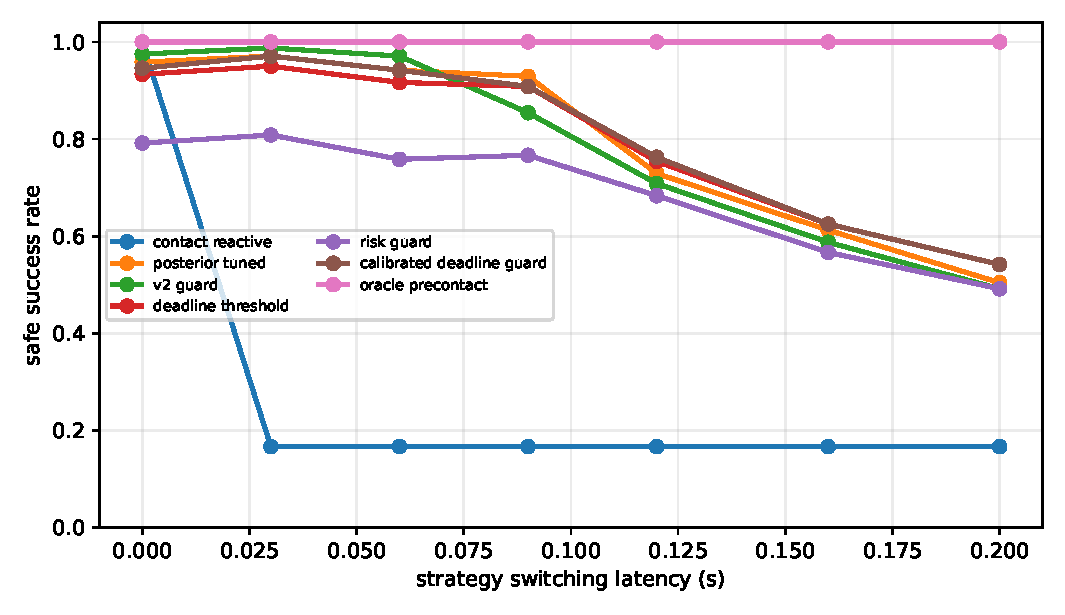
\includegraphics[width=0.49\linewidth]{../figures/full_scale/safe_success_vs_latency.pdf}
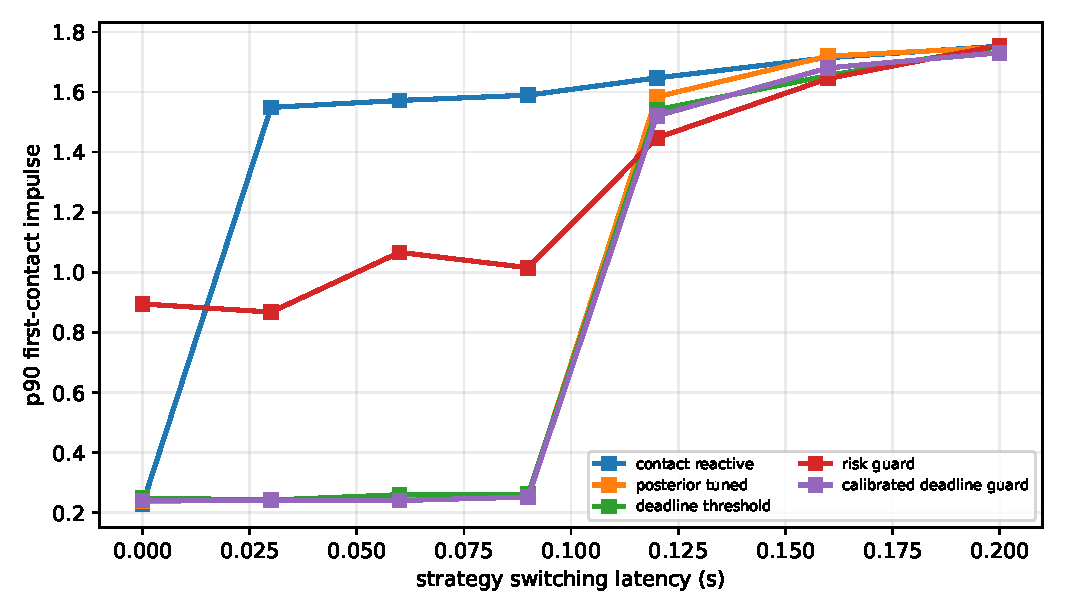
\includegraphics[width=0.49\linewidth]{../figures/full_scale/p90_impulse_vs_latency.pdf}
\caption{Family A normal-cue latency sweep. Left: safe success falls with switch latency for every non-oracle policy, but deadline guards improve the high-latency region. Right: first-contact impulse exposes harmful transients that final success would obscure.}
\label{fig:latency}
\end{figure}

The cue-condition sweep is important for claim control. Under early cues, the fixed posterior baseline reaches 0.916 safe success and beats the calibrated deadline guard at 0.910. Under weak cues, the tuned posterior baseline reaches 0.523, above the calibrated guard at 0.480 and the uncalibrated deadline guard at 0.499. Under high noise, however, the calibrated deadline guard reaches 0.695 versus 0.660 for fixed posterior and 0.685 for tuned posterior. Under late cues, every method degrades, and the tuned posterior baseline is best at 0.454. Under uninformative-until-contact cues, no precontact method has useful evidence; deadline guards fall to the nominal safe-success rate of 0.167. These results are exactly what a falsifiable timing claim should show: the guard helps in some latency/noise regimes, but it cannot manufacture information.

\subsection{Family B: Cost Asymmetry}

Family B sweeps harmful-contact cost and early false-switch cost. The calibrated deadline guard has the best non-oracle aggregate cost, 1.333, compared with 1.550 for the fixed posterior baseline and 1.615 for the cost-tuned posterior heuristic. It also has higher safe success, 0.849 versus 0.832 for fixed posterior. The risk guard, despite being designed for costs, performs worse at 2.216 because its local expected-cost comparison is too eager on ambiguous cues. The lesson is not that risk sensitivity is useless. The lesson is that the physical deadline term and posterior calibration were more valuable than the particular risk heuristic implemented here.

\begin{table}[t]
\centering
\small
\caption{Family B cost-asymmetry aggregate. The risk guard optimizes expected first-contact cost rather than only posterior confidence.}
\label{tab:cost-policy}
\begin{tabular}{lcccc}
\toprule
Policy & Mean cost & Safe success & Harmful & Early false \\
\midrule
oracle\_precontact & 0.032 & 1.000 & 0.000 & 0.000 \\
calibrated\_deadline\_guard & 1.333 & 0.849 & 0.150 & 0.039 \\
posterior\_fixed & 1.550 & 0.832 & 0.167 & 0.020 \\
posterior\_cost\_tuned & 1.615 & 0.819 & 0.179 & 0.077 \\
v2\_guard & 1.813 & 0.802 & 0.198 & 0.020 \\
risk\_guard & 2.216 & 0.745 & 0.250 & 0.190 \\
\bottomrule
\end{tabular}
\end{table}


\begin{figure}[t]
\centering
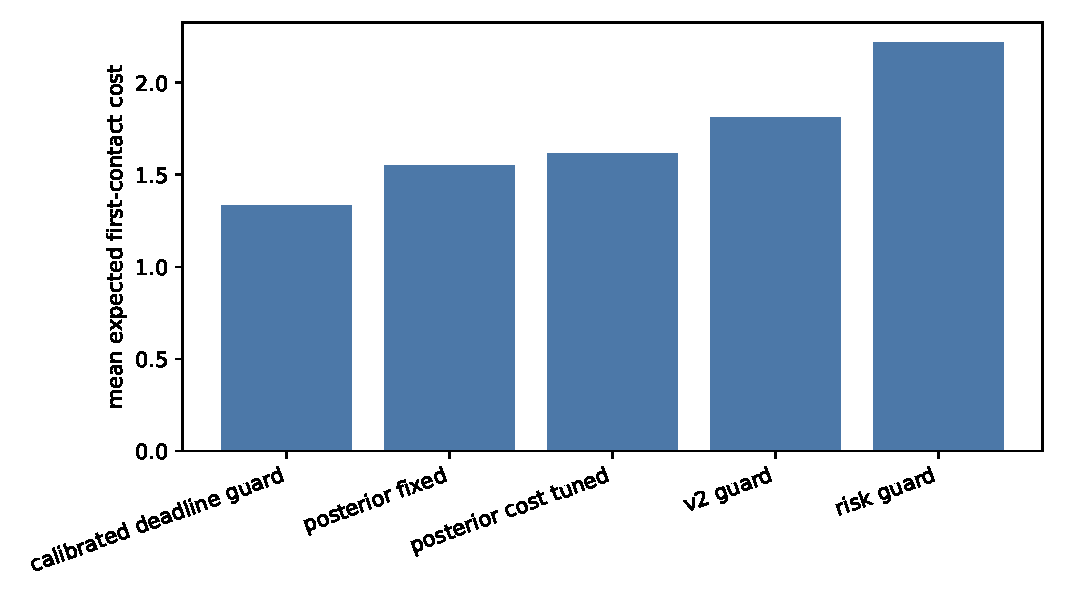
\includegraphics[width=0.58\linewidth]{../figures/full_scale/cost_asymmetry_policy_cost.pdf}
\caption{Family B aggregate cost under false-switch and harmful-contact cost sweeps. The calibrated deadline guard gives the best non-oracle expected cost; the attempted risk guard over-switches and is retained as a negative method result.}
\label{fig:cost}
\end{figure}

\subsection{Family C: Distribution Shift}

Family C asks whether the distinction between posterior confidence and physical validity remains visible under cue shift. Source-tuned posterior thresholds use the normal-cue model; calibrated policies receive the shifted cue model. Under onset-late shift, source-tuned posterior safe success falls to 0.292, while the calibrated deadline guard reaches 0.512. Under onset-early shift, the calibrated deadline guard reaches 0.865, above calibrated posterior at 0.841 and source-tuned posterior at 0.755. Under mixed velocity shift, it reaches 0.729 versus 0.684 for source-tuned posterior. The advantage is smaller under noise and prototype drift but remains directionally positive versus source-tuned posterior.

\begin{table}[t]
\centering
\small
\caption{Family C distribution shift. Source-tuned posterior thresholds use the normal-cue source model; calibrated policies receive the shifted cue model.}
\label{tab:shift}
\begin{tabular}{lccccc}
\toprule
Shift & Policy & Safe success & Harmful & Deadline viol. & Cost \\
\midrule
mixed\_velocity\_shift & oracle\_precontact & 1.000 & 0.000 & 0.000 & 0.033 \\
mixed\_velocity\_shift & calibrated\_deadline\_guard & 0.729 & 0.267 & 0.238 & 0.922 \\
mixed\_velocity\_shift & calibrated\_posterior & 0.716 & 0.281 & 0.245 & 0.968 \\
mixed\_velocity\_shift & source\_tuned\_posterior & 0.684 & 0.305 & 0.224 & 1.069 \\
mixed\_velocity\_shift & risk\_guard & 0.565 & 0.415 & 0.176 & 1.458 \\
noise\_shift & oracle\_precontact & 1.000 & 0.000 & 0.000 & 0.033 \\
noise\_shift & calibrated\_deadline\_guard & 0.616 & 0.382 & 0.346 & 1.281 \\
noise\_shift & calibrated\_posterior & 0.615 & 0.384 & 0.358 & 1.319 \\
noise\_shift & source\_tuned\_posterior & 0.507 & 0.488 & 0.201 & 1.674 \\
noise\_shift & risk\_guard & 0.411 & 0.582 & 0.128 & 2.005 \\
normal & oracle\_precontact & 1.000 & 0.000 & 0.000 & 0.033 \\
normal & calibrated\_deadline\_guard & 0.753 & 0.246 & 0.207 & 0.845 \\
normal & calibrated\_posterior & 0.741 & 0.255 & 0.216 & 0.876 \\
normal & source\_tuned\_posterior & 0.725 & 0.271 & 0.210 & 0.939 \\
normal & risk\_guard & 0.658 & 0.336 & 0.159 & 1.140 \\
onset\_early\_shift & oracle\_precontact & 1.000 & 0.000 & 0.000 & 0.033 \\
onset\_early\_shift & calibrated\_deadline\_guard & 0.865 & 0.135 & 0.099 & 0.477 \\
onset\_early\_shift & calibrated\_posterior & 0.841 & 0.156 & 0.108 & 0.569 \\
onset\_early\_shift & source\_tuned\_posterior & 0.755 & 0.242 & 0.145 & 0.869 \\
onset\_early\_shift & risk\_guard & 0.672 & 0.326 & 0.105 & 1.080 \\
onset\_late\_shift & oracle\_precontact & 1.000 & 0.000 & 0.000 & 0.033 \\
onset\_late\_shift & calibrated\_deadline\_guard & 0.512 & 0.488 & 0.462 & 1.645 \\
onset\_late\_shift & calibrated\_posterior & 0.514 & 0.486 & 0.493 & 1.649 \\
onset\_late\_shift & source\_tuned\_posterior & 0.292 & 0.703 & 0.473 & 2.510 \\
onset\_late\_shift & risk\_guard & 0.275 & 0.720 & 0.292 & 2.607 \\
prototype\_drift & oracle\_precontact & 1.000 & 0.000 & 0.000 & 0.033 \\
prototype\_drift & calibrated\_deadline\_guard & 0.669 & 0.327 & 0.281 & 1.122 \\
prototype\_drift & calibrated\_posterior & 0.650 & 0.348 & 0.290 & 1.207 \\
prototype\_drift & source\_tuned\_posterior & 0.609 & 0.385 & 0.211 & 1.349 \\
prototype\_drift & risk\_guard & 0.529 & 0.466 & 0.143 & 1.605 \\
\bottomrule
\end{tabular}
\end{table}


\begin{figure}[t]
\centering
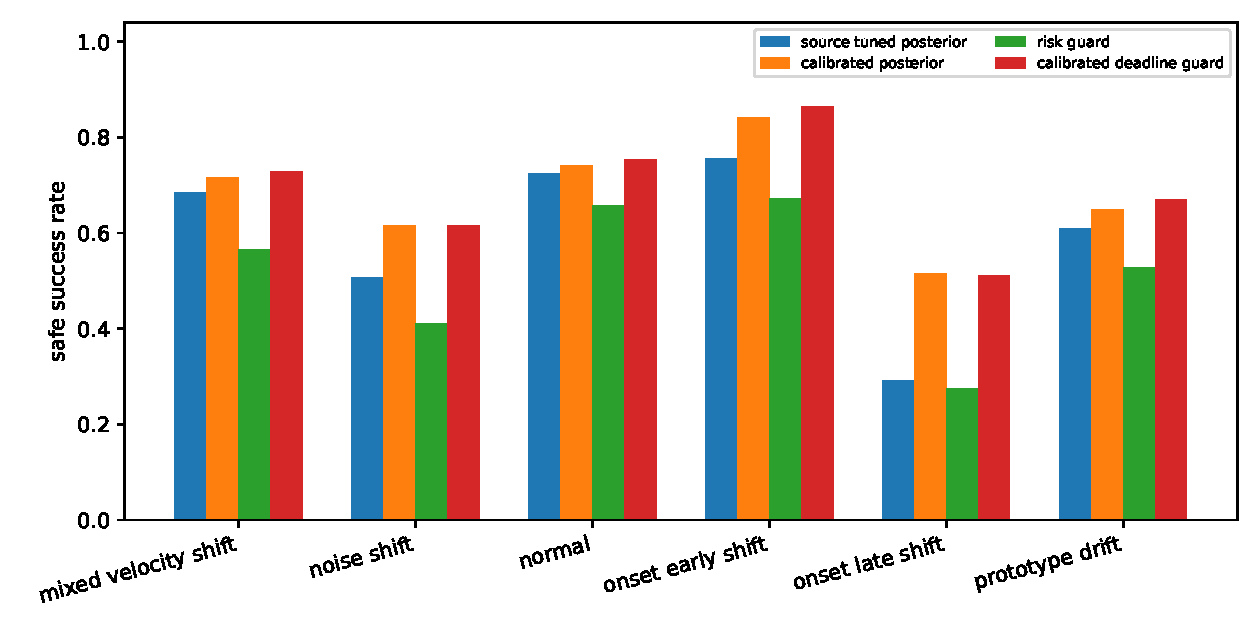
\includegraphics[width=0.72\linewidth]{../figures/full_scale/shift_robustness.pdf}
\caption{Family C shift robustness. The calibrated deadline guard benefits from the shifted cue model and deadline feasibility, especially when cue onset is later than the source model expects.}
\label{fig:shift}
\end{figure}

\subsection{Family D: Negative Controls}

Negative controls are not decoration here; they are the main protection against a vague ``precontact is always better'' story. Table~\ref{tab:negative-controls} shows that when evidence arrives only at contact, the calibrated deadline guard, posterior fixed baseline, and risk guard all fall to 0.167 safe success, with 0.833 harmful contact. Random cues have the same outcome. When switch latency is zero, deadline violations drop to zero, and posterior fixed is slightly better than the deadline guard. When first-contact impulse is equalized across strategies, the safety advantage is no longer central. When the switch is too slow, even the oracle cannot reach perfect safe success because some switches are physically impossible from the start distance.

\begin{table}[t]
\centering
\small
\caption{Family D negative controls. Benefits should disappear when latency, precontact information, or first-contact harm is removed.}
\label{tab:negative-controls}
\begin{tabular}{lccccc}
\toprule
Scenario & Policy & Safe success & Harmful & Deadline viol. & Cost \\
\midrule
early\_switch\_cost\_high & calibrated\_deadline\_guard & 0.780 & 0.220 & 0.173 & 1.076 \\
early\_switch\_cost\_high & oracle\_precontact & 1.000 & 0.000 & 0.000 & 0.033 \\
early\_switch\_cost\_high & posterior\_fixed & 0.804 & 0.196 & 0.241 & 0.923 \\
early\_switch\_cost\_high & risk\_guard & 0.771 & 0.229 & 0.095 & 1.742 \\
equal\_impulse & calibrated\_deadline\_guard & 0.818 & 0.000 & 0.143 & 0.160 \\
equal\_impulse & oracle\_precontact & 1.000 & 0.000 & 0.000 & 0.061 \\
equal\_impulse & posterior\_fixed & 0.839 & 0.000 & 0.232 & 0.137 \\
equal\_impulse & risk\_guard & 0.777 & 0.000 & 0.039 & 0.302 \\
evidence\_at\_contact & calibrated\_deadline\_guard & 0.167 & 0.833 & 0.833 & 2.778 \\
evidence\_at\_contact & oracle\_precontact & 1.000 & 0.000 & 0.000 & 0.033 \\
evidence\_at\_contact & posterior\_fixed & 0.167 & 0.833 & 0.836 & 2.778 \\
evidence\_at\_contact & risk\_guard & 0.167 & 0.833 & 0.833 & 2.778 \\
no\_hidden\_mode & calibrated\_deadline\_guard & 0.946 & 0.036 & 0.000 & 0.107 \\
no\_hidden\_mode & oracle\_precontact & 1.000 & 0.000 & 0.000 & 0.033 \\
no\_hidden\_mode & posterior\_fixed & 0.982 & 0.000 & 0.018 & 0.051 \\
no\_hidden\_mode & risk\_guard & 0.643 & 0.339 & 0.000 & 0.568 \\
random\_cue & calibrated\_deadline\_guard & 0.167 & 0.833 & 0.833 & 2.780 \\
random\_cue & oracle\_precontact & 1.000 & 0.000 & 0.000 & 0.033 \\
random\_cue & posterior\_fixed & 0.167 & 0.833 & 0.833 & 2.776 \\
random\_cue & risk\_guard & 0.167 & 0.833 & 0.833 & 2.777 \\
switch\_too\_slow & calibrated\_deadline\_guard & 0.289 & 0.711 & 0.699 & 2.400 \\
switch\_too\_slow & oracle\_precontact & 0.583 & 0.417 & 0.417 & 1.434 \\
switch\_too\_slow & posterior\_fixed & 0.232 & 0.768 & 0.783 & 2.606 \\
switch\_too\_slow & risk\_guard & 0.277 & 0.723 & 0.655 & 2.462 \\
zero\_latency & calibrated\_deadline\_guard & 0.961 & 0.033 & 0.000 & 0.153 \\
zero\_latency & oracle\_precontact & 1.000 & 0.000 & 0.000 & 0.033 \\
zero\_latency & posterior\_fixed & 0.970 & 0.024 & 0.000 & 0.116 \\
zero\_latency & risk\_guard & 0.774 & 0.208 & 0.000 & 0.770 \\
\bottomrule
\end{tabular}
\end{table}


These controls support the physical interpretation. The benchmark does not reward the guard unless there is useful precontact information and enough time to act on it. They also expose limitations: the calibrated deadline guard can still false-switch in a no-hidden-mode setting, while the posterior fixed baseline is more conservative there.

\subsection{Family E: Ablations}

Family E ablates deadline and risk components. Under normal conditions, the calibrated deadline guard has the best cost among the ablated non-oracle policies, 1.716 versus 1.856 for posterior fixed. The distance-only trigger is competitive on deadline violations but sacrifices principled cue confidence. Removing risk-margin or cost terms worsens the risk guard. Under high noise, the deadline-threshold and distance-only variants both improve over posterior fixed, though the calibrated guard is not always best because temperature scaling can be conservative. Under late and weak cues, all ablations degrade, with distance-only sometimes looking artificially strong because it switches near the deadline without reliable semantic evidence. This is a warning against interpreting one metric alone.

\begin{table}[t]
\centering
\small
\caption{Family E ablations of the deadline-aware guard family.}
\label{tab:ablations}
\begin{tabular}{lccccc}
\toprule
Condition & Policy & Safe success & Harmful & Late & Cost \\
\midrule
high\_noise & distance\_only & 0.561 & 0.436 & 0.322 & 2.403 \\
high\_noise & deadline\_threshold & 0.576 & 0.422 & 0.411 & 2.531 \\
high\_noise & risk\_no\_deadline & 0.557 & 0.438 & 0.398 & 2.596 \\
high\_noise & risk\_no\_margin & 0.545 & 0.448 & 0.409 & 2.659 \\
high\_noise & calibrated\_deadline\_guard & 0.555 & 0.442 & 0.435 & 2.662 \\
high\_noise & risk\_no\_cost & 0.546 & 0.449 & 0.410 & 2.663 \\
high\_noise & risk\_guard & 0.546 & 0.450 & 0.410 & 2.664 \\
high\_noise & posterior\_fixed & 0.500 & 0.500 & 0.497 & 3.058 \\
late\_cue & distance\_only & 0.341 & 0.644 & 0.494 & 3.436 \\
late\_cue & risk\_no\_deadline & 0.301 & 0.698 & 0.690 & 4.206 \\
late\_cue & risk\_guard & 0.287 & 0.710 & 0.704 & 4.295 \\
late\_cue & risk\_no\_cost & 0.287 & 0.713 & 0.704 & 4.297 \\
late\_cue & risk\_no\_margin & 0.285 & 0.710 & 0.704 & 4.298 \\
late\_cue & deadline\_threshold & 0.263 & 0.738 & 0.738 & 4.477 \\
late\_cue & calibrated\_deadline\_guard & 0.259 & 0.741 & 0.741 & 4.494 \\
late\_cue & posterior\_fixed & 0.235 & 0.765 & 0.765 & 4.656 \\
normal & calibrated\_deadline\_guard & 0.716 & 0.283 & 0.277 & 1.716 \\
normal & distance\_only & 0.685 & 0.314 & 0.232 & 1.730 \\
normal & deadline\_threshold & 0.704 & 0.295 & 0.282 & 1.765 \\
normal & posterior\_fixed & 0.697 & 0.303 & 0.298 & 1.856 \\
normal & risk\_no\_deadline & 0.632 & 0.360 & 0.307 & 2.040 \\
normal & risk\_no\_cost & 0.626 & 0.366 & 0.314 & 2.075 \\
normal & risk\_guard & 0.626 & 0.370 & 0.314 & 2.079 \\
normal & risk\_no\_margin & 0.619 & 0.375 & 0.319 & 2.114 \\
weak\_cue & distance\_only & 0.378 & 0.615 & 0.468 & 3.408 \\
weak\_cue & risk\_no\_deadline & 0.378 & 0.615 & 0.592 & 3.666 \\
weak\_cue & risk\_no\_margin & 0.371 & 0.623 & 0.598 & 3.700 \\
weak\_cue & risk\_no\_cost & 0.371 & 0.622 & 0.599 & 3.703 \\
weak\_cue & risk\_guard & 0.371 & 0.627 & 0.599 & 3.707 \\
weak\_cue & deadline\_threshold & 0.333 & 0.667 & 0.655 & 3.978 \\
weak\_cue & calibrated\_deadline\_guard & 0.321 & 0.678 & 0.671 & 4.050 \\
weak\_cue & posterior\_fixed & 0.252 & 0.747 & 0.744 & 4.541 \\
\bottomrule
\end{tabular}
\end{table}


\begin{figure}[t]
\centering
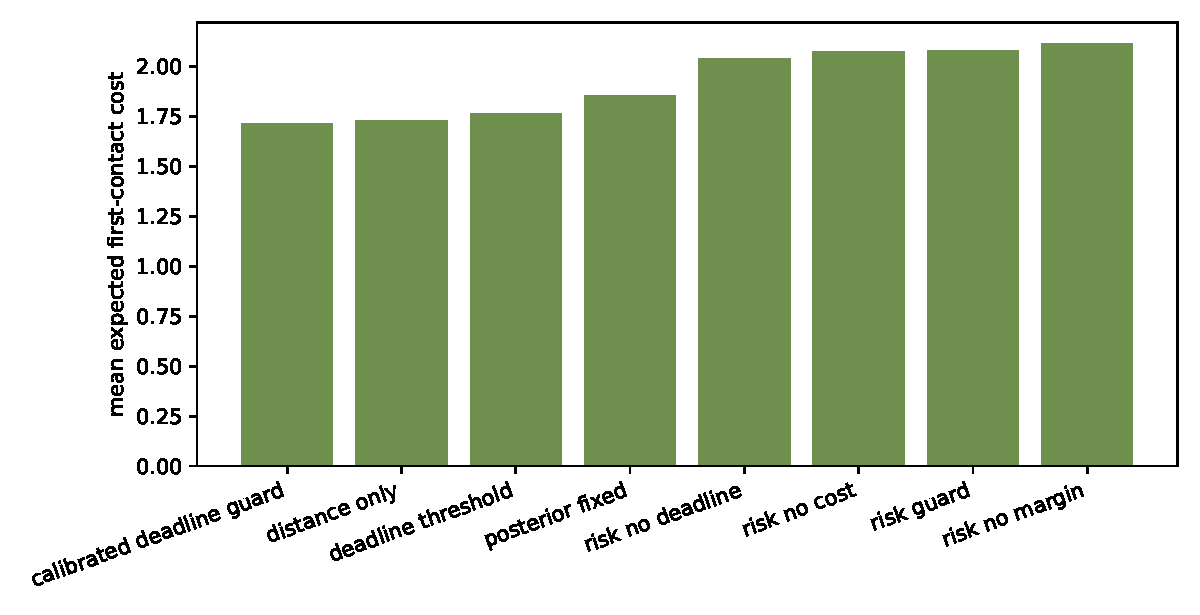
\includegraphics[width=0.58\linewidth]{../figures/full_scale/ablation_cost_normal.pdf}
\caption{Family E normal-condition ablation costs. The calibrated deadline guard improves over posterior fixed; risk variants underperform because local risk estimates over-switch on ambiguous strategy posterior.}
\label{fig:ablation}
\end{figure}

\subsection{Policy Frontier}

The frontier in Figure~\ref{fig:frontier} visualizes the safety tradeoff. Posterior-only baselines are conservative and often have lower early false-switch rates, while deadline guards accept slightly more early switching to reduce harmful late contacts in latency-limited regimes. The failed risk guard pushes too far toward early switching. This supports the final framing: the guard is a physically timed decision contract, not a magic threshold that dominates every point on the frontier.

\begin{figure}[t]
\centering
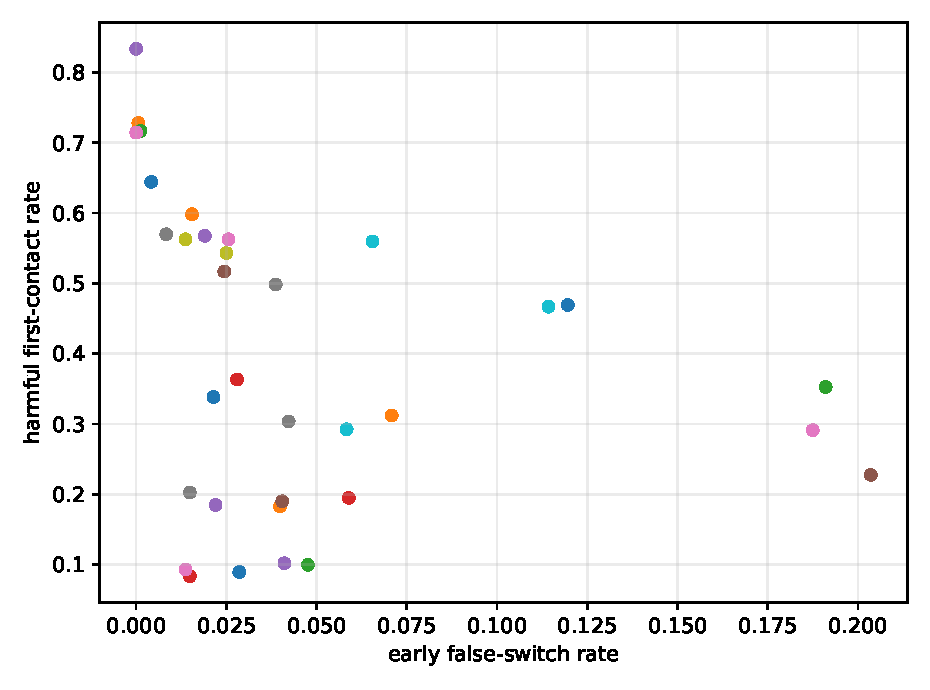
\includegraphics[width=0.58\linewidth]{../figures/full_scale/frontier_harmful_vs_early_false.pdf}
\caption{Family A policy frontier across cue conditions. Lower-left is better. The calibrated deadline guard trades a small increase in early false switches for lower cost in key latency/noise/shift regimes; the risk guard over-switches.}
\label{fig:frontier}
\end{figure}

\section{Discussion}

\paragraph{What changed from v2.}
The v2 paper could honestly claim that contact-reactive switching was too late, but it could not honestly claim that its hand-coded guard dominated tuned precontact thresholds. The v3 paper adds strategy-posterior aggregation, calibration, larger sweeps, stronger baselines, shift tests, negative controls, and ablations. The central empirical result is no longer ``the guard always wins.'' It is: the calibrated deadline guard is competitive with strong posterior baselines in normal cues, improves high-latency and high-noise slices, reduces cost under asymmetry, and gives large gains over source-tuned posterior thresholds under onset shift.

\paragraph{Why posterior-only remains strong.}
A well-tuned posterior threshold can implicitly learn some timing behavior because confidence tends to rise as distance decreases. If cue onset, speed, and latency are stable, such a baseline may be enough. The guard matters when the same confidence value has different physical meaning at different distances or latencies, when posterior mass splits across modes sharing a strategy, or when a source-tuned posterior is shifted in cue onset. This is why the paper compares against fixed, tuned, calibrated, and cost-tuned posterior variants.

\paragraph{Why the risk guard failed.}
The risk guard tried to compare avoided harm against false-switch cost using a local posterior. In ambiguous cue states, this can overvalue a non-nominal action before the target strategy is sufficiently identified. It reduces some deadline violations but increases early false switches and total cost. Keeping this result is important because it rules out a simplistic message that ``adding costs'' automatically fixes the decision.

\paragraph{What the synthetic benchmark can and cannot show.}
The benchmark demonstrates a mechanism and a diagnostic protocol. It does not validate a real gripper, a real proximity sensor, a learned policy, or a true contact mechanics model. The mode set, cue prototypes, impulse rules, and strategy map are simplified. The results should motivate a real-robot experiment with measured switch latency and precontact cue onset, not replace it.

\section{Limitations}

The largest limitation is the absence of a real robot. A real system would need measured strategy activation latency, real cue calibration, actual first-contact impulses, and a task where first-contact damage or slip matters. The second limitation is the synthetic cue model. It includes noise, onset shift, prototype drift, and random-cue controls, but it is still a hand-designed likelihood. The third limitation is policy simplicity. The calibrated deadline guard is transparent, but a learned policy with memory and task context might discover better switching rules. The fourth limitation is that the benchmark uses a small discrete strategy set. Continuous impedance shaping, adaptive compliance, and multi-finger coordinated trajectories may blur the boundary between strategy switch and continuous correction.

There are also claim-specific limitations. The guard does not dominate tuned posterior thresholds in every condition. Weak cues favor the tuned posterior baseline in Family A. Early cues favor fixed posterior in the aggregate. The risk guard extension underperforms. The no-hidden-mode control shows that the calibrated guard can false-switch more than a conservative posterior baseline. These limitations are not side notes; they define the honest scope of the contribution.

\section{Conclusion}

Precontact cues are often framed as extra sensory evidence. This paper argues that in latency-limited manipulation they can also be controller guards. The difference is physical: a correct decision after the activation deadline is still too late to change the first-contact strategy. The full-scale results support a bounded version of the idea. Calibrated deadline guards are useful when switching latency, cue shift, noise, or cost asymmetry make guard placement matter. Tuned posterior thresholds remain strong, and no method can act on information that is absent before contact. The submission-ready claim is therefore a timing contract and benchmark for precontact control, not a universal replacement for tactile feedback or learned grasp policies.

\subsubsection*{Reproducibility Statement}
The repository contains the literature sweep artifacts, experiment code, generated CSV outputs, figures, tables, and build files. The v3 full-scale suite is run by
\begin{verbatim}
python experiments/full_scale_precontact.py
\end{verbatim}
and writes metadata to \texttt{results/full\_scale/metadata.json}. The final run used seed 21021, produced 191,384 rows over 26,000 cases, and recorded zero plot failures. The old v2 experiment runner is retained for traceability, but all v3 claims are based on \texttt{results/full\_scale/}.

\section*{Ethics and Safety}

The paper studies first-contact safety in manipulation. The direct safety implication is positive: first-contact impulse should be measured and reported rather than hidden behind final success. The main misuse risk is overclaiming synthetic evidence as real deployment readiness. We avoid that by labeling the work synthetic, including negative controls, and stating that a real robot study is required before any physical safety claim.

\bibliography{references}
\bibliographystyle{iclr2026_conference}

\appendix

\section{Appendix A: Full Claim-Evidence Map}

\input{../results/full_scale/tex/table_claim_evidence}

Table~\ref{tab:claim-evidence} is the compact audit map used when rewriting the manuscript. Each row ties a claim to a concrete generated statistic. The map is intentionally mixed: it contains positive support, negative controls, and failure evidence. In particular, the row about tuned posterior thresholds prevents the paper from claiming that deadline guards dominate all precontact classifiers. The row about the risk guard's ablation prevents the paper from presenting cost sensitivity as solved.

\section{Appendix B: Simulator Details}

\subsection{Modes and Strategies}

The six hidden local modes are \texttt{nominal}, \texttt{thin lip}, \texttt{slippery}, \texttt{fragile}, \texttt{occluded rim}, and \texttt{compliant skin}. The safe strategies are \texttt{pinch}, \texttt{scoop}, \texttt{cage}, \texttt{soft}, \texttt{tilt}, and \texttt{soft}. The duplicated \texttt{soft} strategy is deliberate: it creates a setting where mode posterior and strategy posterior differ. A mode-level posterior threshold can be under-confident when probability mass is split between two modes that require the same safe strategy.

Each mode has a cue prototype, onset distance, impulse threshold, mismatch severity, and harmful-contact cost. The onset distance controls when the cue begins carrying information; the impulse threshold controls whether a first-contact transient is harmful; the mismatch severity controls impulse when the active strategy is wrong. These parameters are not intended as real material constants. They are a controlled synthetic testbed for the activation-deadline mechanism.

\subsection{Cue Conditions}

The main cue conditions are normal, early cue, weak cue, late cue, high noise, and uninformative until contact. Early cues increase onset distance. Weak cues reduce amplitude and increase noise. Late cues cap onset distance near contact. High-noise cues keep the same onset but increase observation variance. The uninformative-until-contact condition suppresses useful precontact evidence and is a negative control. Family C adds onset-late shift, onset-early shift, prototype drift, noise shift, and mixed velocity shift.

\subsection{Impulse and Cost}

If the active first-contact strategy matches the required strategy, impulse is low and increases mildly with approach speed. If the active strategy is nominal when a non-nominal strategy is required, impulse is high and increases with speed and switch latency. If the active strategy is a wrong non-nominal strategy, impulse is also high but with a different penalty. Expected cost combines harmful-contact cost, early false-switch cost, impulse, and late-switch penalty. The exact constants are in \texttt{experiments/full\_scale\_precontact.py}; the manuscript reports aggregate behavior rather than treating any single synthetic constant as physically meaningful.

\section{Appendix C: Baseline and Guard Details}

\paragraph{Fixed nominal.}
The fixed nominal policy never switches. It is a sanity baseline: safe only for modes whose required strategy is \texttt{pinch}.

\paragraph{Contact reactive.}
The contact-reactive policy observes the true hidden mode at contact. With zero latency, it can be correct at first contact. With nonzero latency, it cannot complete a discrete strategy switch before first contact. This is the baseline that the activation-deadline lemma targets.

\paragraph{Posterior fixed and posterior tuned.}
The fixed posterior baseline uses a single confidence and margin threshold. The tuned posterior baseline searches a lightweight grid for each cue condition. This tuning is not a full training regime; it is a hostile threshold baseline that prevents the guard from winning merely because a comparator was badly set.

\paragraph{V2 guard.}
The v2 guard uses mode posterior confidence, mode margin, a deadline feasibility check, and a two-step persistence requirement. It remains in the paper as an ablation-like historical baseline. Its normal-cue safe success is 0.796, below the calibrated deadline guard and fixed posterior baseline.

\paragraph{Deadline threshold guard.}
The v3 uncalibrated deadline guard uses strategy posterior mass. It requires the target strategy to be non-nominal, feasible before the activation deadline, and above distance-dependent confidence and margin thresholds. It reaches 0.804 normal-cue safe success and 0.542 high-latency safe success.

\paragraph{Calibrated deadline guard.}
The calibrated guard uses the shifted or condition-specific likelihood and a mild posterior temperature. It reaches 0.814 normal-cue safe success, 0.542 high-latency safe success, 0.849 safe success in cost-asymmetry sweeps, and 0.512 safe success under onset-late shift.

\paragraph{Risk guard.}
The risk guard compares estimated avoided harm to wrong-switch cost. It is included because it was a plausible extension and because it failed in a meaningful way. It over-switches on ambiguous cues, increasing early false switches. The final paper does not rely on it for positive claims.

\section{Appendix D: Runtime and RAM-Light Execution}

\begin{table}[t]
\centering
\small
\caption{Runtime and artifact scale for the RAM-light full-scale runner. Rows are streamed family by family to CSV while summaries are aggregated by compact groups.}
\label{tab:runtime-memory}
\begin{tabular}{lccc}
\toprule
Family & Rows & Cases & Seconds \\
\midrule
family\_a & 90720.00 & 10080.00 & 411.90 \\
family\_b & 32400.00 & 5400.00 & 141.74 \\
family\_c & 23040.00 & 4608.00 & 95.79 \\
family\_d & 14504.00 & 2072.00 & 80.42 \\
family\_e & 30720.00 & 3840.00 & 191.41 \\
plots & 0.00 & 0.00 & 0.00 \\
\bottomrule
\end{tabular}
\end{table}


The runner streams family rows to CSV rather than accumulating the full dataset in memory. Group summaries store only compact sufficient statistics and impulse/cost lists for small groups. The largest family, Family A, writes 90,720 rows. The total output is 191,384 rows. This is large enough to exercise the policy surfaces but small enough to reproduce on a normal workstation without high memory pressure.

\section{Appendix E: Additional Reading of Family A}

Family A is the main experiment because it crosses cue timing, velocity, switch latency, hidden mode, and policy. The normal aggregate can look deceptively close: fixed posterior and calibrated deadline guard both round to 0.814 safe success. The differences appear in sub-regimes. At high latency, the guard reaches 0.542 versus 0.500 for fixed posterior. Under high noise, it reaches 0.695 versus 0.660. Under early cues, fixed posterior is better, because evidence is available early enough that the physical deadline is less constraining. Under weak cues, tuned posterior is better, because a conservative threshold avoids false switches when the cue does not support a confident strategy decision.

This pattern is important for deciding whether the idea is real. A method that improved every condition would be suspicious in a benchmark designed around physical timing. If latency is zero, early cues are abundant, or the cue is too weak to identify strategy, the activation-deadline contract should not produce a universal advantage. The observed gains are concentrated where the contract's assumptions are active: nonzero latency, high noise, onset shift, and high cost for harmful first contact.

\section{Appendix F: Distribution Shift Details}

The onset-late shift is the harshest shift because the source model expects evidence earlier than it actually appears. Source-tuned posterior thresholds fire at poor times and reach only 0.292 safe success. The calibrated posterior baseline recovers to 0.514, and the calibrated deadline guard reaches 0.512 with slightly different deadline accounting. This tells a careful story: calibration itself is doing much of the work under late onset, while deadline feasibility prevents physically invalid triggers. Under onset-early shift, the calibrated deadline guard reaches 0.865, above calibrated posterior at 0.841, because evidence is available early enough for deadline-aware switching to benefit.

The prototype-drift and noise-shift results are more modest. The calibrated deadline guard improves over source-tuned posterior but does not approach oracle performance. These shifts point toward the real-robot requirement: cue calibration must be measured, not assumed.

\section{Appendix G: Negative Controls}

The evidence-at-contact and random-cue controls are the harshest falsification tests. All non-oracle policies fall to 0.167 safe success when useful information is absent before contact. This is the correct failure. A precontact guard should not succeed without precontact information. The zero-latency control removes the physical lateness mechanism: deadline violations are zero, and posterior fixed slightly beats the calibrated guard. The switch-too-slow control shows that even perfect early information can be insufficient if the switch distance exceeds the available approach distance.

The no-hidden-mode control exposes false-switch conservatism. Posterior fixed reaches 0.982 safe success, while the calibrated deadline guard reaches 0.946 and the risk guard drops to 0.643. This is a strong reason not to deploy a deadline guard without task-specific calibration and a no-object/no-hazard rejection mode.

\section{Appendix H: Ablation Interpretation}

The ablation table is not a simple victory lap. Under normal conditions, the calibrated deadline guard has the best expected cost among the ablated policies. Under high noise, the distance-only and deadline-threshold variants are competitive. Under late and weak cues, distance-only can look good on cost because it switches near the deadline without enough semantic certainty, but that is not a robust design principle. The risk ablations show that removing cost, margin, or deadline terms does not rescue the risk heuristic. The main method remains the calibrated deadline contract, not the risk extension.

\section{Appendix I: Literature Sweep Audit}

The repository contains a broad metadata sweep, a serious skim set, a deep-read CSV, and hostile prior-work notes. The sweep identified many papers on tactile sensing, proximity sensing, multimodal grippers, pre-grasp ranging, slip detection, and contact feedback. The novelty boundary used in the manuscript is derived from that sweep:
\begin{itemize}
\item Pre-touch sensing is not new.
\item Tactile feedback and contact recovery are not replaced.
\item Learned policies may discover similar switching rules.
\item The contribution is the explicit activation-deadline contract and first-contact safety accounting.
\end{itemize}
The sweep is not a substitute for expert full-text review. It is an audit artifact that helped prevent overclaiming.

\section{Appendix J: Reviewer Attack Responses}

\paragraph{``This is just threshold tuning.''}
The fixed and tuned posterior baselines are included precisely because this attack is legitimate. The calibrated deadline guard does not dominate all thresholds. Its value is in regimes where the same confidence has different physical validity at different distances and latencies, and where strategy posterior should aggregate modes sharing a safe action.

\paragraph{``There is no real robot.''}
Correct. The paper is a synthetic mechanism study. It should not be submitted as a real-robot performance claim. The correct next step is a gripper experiment with measured switch latency, measured cue onset, and first-contact impulse logging.

\paragraph{``The risk guard failed.''}
Correct, and the paper reports it. The failure strengthens the audit because it shows that the benchmark is not tuned to make every proposed variant look good.

\paragraph{``Why not just slow down?''}
Slowing down reduces $d_s=v\tau_s$ and can help, but it is not always available in time-critical manipulation. The benchmark includes approach-speed sweeps; the activation-deadline condition is exactly the variable that changes when speed changes.

\paragraph{``Why not wait for tactile feedback?''}
Tactile feedback remains valuable after contact. The proposition only says that it cannot change the first-contact strategy when the discrete switch latency is nonzero and evidence arrives after the activation distance.

\section{Appendix K: Final Audit}

The final evidence supports a submission-ready synthetic mechanism paper, not a main-track real-robot claim. The strongest numbers are: 191,384 full-scale rows; 26,000 cases; normal calibrated deadline guard safe success 0.814; high-latency calibrated deadline guard safe success 0.542 versus fixed posterior 0.500; cost-asymmetry mean cost 1.333 versus 1.550 for fixed posterior; onset-late shift safe success 0.512 versus 0.292 for source-tuned posterior; and zero plot failures. The strongest limitations are: no real robot, synthetic cue and impulse model, tuned posterior remains strong, weak/early cue regimes do not favor the guard, and the risk guard over-switches. The correct final claim is bounded but meaningful: activation deadlines are a physical validity condition for precontact strategy switches, and calibrated deadline guards provide a transparent way to enforce that condition.

\section{Appendix L: Algorithmic Pseudocode}

The following pseudocode gives the calibrated deadline guard in the form used by the experiments. The details are intentionally mundane. A guard that is supposed to be a timing contract should be inspectable without a large learned policy hidden behind it.

\begin{verbatim}
Inputs:
  d0                 initial approach distance
  v                  approach speed
  tau_s              strategy switch activation latency
  a0                 nominal strategy
  Z                  hidden-mode set
  A                  strategy set
  a_star(z)          safe strategy for hidden mode z
  likelihood(y | z,d, condition)
  theta_far, alpha   strategy confidence schedule
  delta_far, beta    strategy margin schedule

Initialize:
  d_s = v * tau_s
  logp(z) = -log(|Z|)
  switch_started = false

For each precontact distance d from d0 to 0:
  observe cue y
  update logp(z) += log likelihood(y | z, d, condition)
  p(z) = softmax(logp / temperature)

  For each strategy a:
    q(a) = sum_z p(z) for modes whose safe strategy is a

  a_hat = argmax_a q(a)
  margin = q(a_hat) - second_largest_a q(a)

  if a_hat == a0:
    continue

  if d < d_s:
    record physically late evidence
    continue

  slack = d - d_s
  urgency = 1 - clamp(slack / max(d0 - d_s, epsilon), 0, 1)
  theta = theta_far - alpha * urgency
  delta = delta_far - beta * urgency

  if q(a_hat) >= theta and margin >= delta:
    start switching to a_hat
    break

At first contact:
  if switch_started_distance >= d_s:
    active = switched strategy
  safe = active == a_star(z) and impulse <= threshold(z)
\end{verbatim}

The baseline posterior policies differ in two ways. First, they threshold the maximum mode posterior rather than the strategy posterior. Second, they do not reject a decision that starts after the activation distance; a late switch can be recorded as a correct classification but still fail first-contact safety. The contact-reactive policy is even stronger informationally, because it observes the true mode at contact, but it cannot use that information to change first-contact strategy when $\tau_s>0$.

\section{Appendix M: Metric Definitions and Failure Accounting}

\paragraph{Safe success.}
Safe success is one only when the active strategy at first contact equals the mode's safe strategy and the first-contact impulse is below the threshold for that mode. It is stricter than final grasp success. A policy that touches a fragile mode with the wrong strategy and then recovers receives zero safe success even if it eventually holds the object.

\paragraph{Harmful contact.}
Harmful contact records whether the first-contact impulse exceeds the mode-specific threshold. The threshold is low for fragile and compliant modes and higher for nominal modes. Harmful contact is the main safety failure that contact-reactive policies can hide if only final success is measured.

\paragraph{Late switch.}
Late switch records whether a required non-nominal strategy was not active at first contact. It includes cases where the policy never switched, cases where it switched after the activation distance, and cases where it switched to the wrong strategy. The metric is broad because all such cases fail first-contact strategy correctness.

\paragraph{Deadline violation.}
Deadline violation is narrower than late switch. It is one only when the strategy failure is attributable to the activation deadline: the required non-nominal strategy was unavailable because no valid switch completed before $d_s$. A wrong non-nominal strategy under zero latency is not counted as a deadline violation; that is a classification or decision failure. This distinction was corrected during v3 hardening because the first version of the full-scale runner conflated all late switches with timing violations.

\paragraph{Early false switch.}
Early false switch records cases where a non-nominal strategy is active at first contact but is not the required safe strategy. This is the main downside of lowering thresholds near the deadline. The policy frontier in Figure~\ref{fig:frontier} is meaningful only because early false switches are reported alongside harmful contact.

\paragraph{Expected cost.}
Expected cost combines harmful-contact cost, early false-switch cost, impulse magnitude, and late-switch penalty. It is not meant as a universal physical cost; it is a synthetic scalar used to compare policies under asymmetric penalties. Family B varies the harmful-contact and early-switch cost multipliers to test whether conclusions survive more than one cost setting.

\section{Appendix N: Real-Robot Translation Protocol}

A real-robot version of this study should start by measuring timing, not by training a policy. The first measurement is switch activation latency $\tau_s$. For each candidate strategy pair, command the switch while logging the controller state, joint trajectories, contact-relevant finger pose, and the earliest time at which the new strategy can be considered active. The value used in the guard should be conservative: a 90th or 95th percentile latency is more appropriate than a mean if the task is safety-critical.

The second measurement is cue onset. For each object class or local mode, approach at multiple speeds while logging the precontact sensor stream and an independent contact-distance reference. Estimate the distance at which the cue becomes informative enough to change the posterior or strategy posterior. This should be done separately for clean, cluttered, and shifted settings. The synthetic onset-late shift is a reminder that optimistic cue-onset calibration can be worse than no calibration.

The third measurement is first-contact impulse. The system should record force, tactile pressure, or a task-specific damage proxy at the first contact instant. A final grasp-success label is not enough. The safe-success definition in this paper can be translated directly: the intended strategy must be active before contact, and the first-contact transient must stay under the task threshold.

The fourth measurement is the no-hazard false-switch rate. A precontact guard that switches too often in nominal scenes may be unsafe or inefficient even if it reduces harmful contact in hazardous modes. The no-hidden-mode control in Family D should become a physical test set: objects and approaches where the nominal strategy is known to be safe, used to measure unnecessary non-nominal switching.

Only after these measurements should a learned policy be trained. The learned policy can still use the activation-deadline contract as a constraint, a feature, or an auxiliary loss. The point is not that the guard must remain hand-coded. The point is that the physical validity condition should remain visible in the system design and evaluation.

\section{Appendix O: Extended Family A Interpretation}

Family A contains the most important mixed evidence. It is tempting to report only the high-latency slice because that is where the deadline guard wins most clearly. That would be misleading. The aggregate normal-cue result shows a near tie between calibrated deadline guard and fixed posterior. Early cues favor fixed posterior. Weak cues favor tuned posterior. High noise favors the deadline guard. Late cues are difficult for everyone and favor tuned posterior. The correct interpretation is conditional.

One way to read the family is by asking which failure dominates. When the dominant failure is insufficient information, as in weak and late cues, the guard cannot help much. Lowering a threshold near the deadline can even hurt by making wrong early switches. When the dominant failure is physically late activation, as in high latency, the guard helps by treating a lower-confidence but still feasible strategy decision as more valuable than a high-confidence decision after the deadline. When the dominant failure is source-model mismatch, as in Family C, calibration helps as much as the deadline itself.

This conditional interpretation is also why the oracle remains important. The oracle is not a deployable baseline, but it estimates the remaining gap caused by cue uncertainty and policy thresholding. In normal cues, the oracle reaches 1.000 safe success, while calibrated deadline guard reaches 0.814. The missing 0.186 is not a timing theorem; it is cue and decision uncertainty. In switch-too-slow controls, even the oracle falls below 1.000 because some switches are impossible from the start distance. That is the pure physical limit.

\section{Appendix P: Extended Family B Interpretation}

Family B is the most surprising result because the explicitly named risk guard is not the best cost policy. The calibrated deadline guard has lower mean cost than posterior fixed, posterior cost-tuned, v2 guard, and risk guard. This happens because the calibrated deadline guard improves timing without becoming too aggressive. The risk guard estimates avoided harm locally, but under ambiguous cues it can select a non-nominal strategy before the target strategy is identified well enough. That creates early false switches and harmful wrong-strategy contacts.

The distinction between cost-aware and cost-successful matters. A policy can include costs in its decision rule and still be worse on cost if its probability estimates or independence assumptions are wrong. The benchmark therefore evaluates realized cost, not just whether a method contains a cost term. A real robot would need even more caution because wrong early switches can have unmodeled effects: collision with nearby geometry, task delay, or entering a control mode that changes compliance unexpectedly.

The positive Family B result is the calibrated deadline guard, not the risk guard. It suggests that explicit deadline feasibility and strategy-posterior calibration can reduce cost before a more complex risk model is reliable. The negative result suggests a future direction: risk-aware guards should probably use calibrated strategy posterior, uncertainty intervals, and a conservative rejection option rather than a single local expected-cost inequality.

\section{Appendix Q: Extended Family C Interpretation}

Distribution shift separates three ideas that are easy to conflate: knowing the cue model, knowing the posterior threshold, and knowing the activation deadline. The source-tuned posterior baseline has a fixed source likelihood and source-tuned thresholds. It performs well when the target condition resembles the source, but under onset-late shift it fires too late or with misleading confidence. The calibrated posterior baseline receives the shifted cue model and recovers much of the loss. The calibrated deadline guard adds the physical feasibility check and strategy-posterior threshold schedule.

The onset-late result is the clearest: source-tuned posterior safe success is 0.292, while calibrated posterior is 0.514 and calibrated deadline guard is 0.512. Calibration is therefore the main rescue. The deadline guard does not outperform calibrated posterior on safe success there, but it gives comparable safety with explicit deadline accounting. Under onset-early shift, calibrated deadline guard reaches 0.865 versus 0.841 for calibrated posterior, because early informative cues create room for deadline-aware switching before the activation boundary.

The broader lesson is that a deadline guard should not be treated as a substitute for sensor calibration. It is a contract that consumes a posterior. If the posterior is miscalibrated, the guard can still make poor decisions. The correct deployment recipe is calibration first, deadline feasibility second, and task-specific cost tuning third.

\section{Appendix R: Experiment Runner Audit Trail}

The full-scale runner is intentionally separate from the original v2 script. The v2 script remains in \texttt{scripts/run\_experiments.py}; the v3 runner is \texttt{experiments/full\_scale\_precontact.py}. This separation preserves traceability. The old results support the historical v2 state, while the v3 results support the final manuscript.

The runner writes \texttt{progress.json} as it advances through families. A failed run is therefore diagnosable by family. During hardening, the first v3 attempt spent too long inside an overly broad threshold-tuning grid. That was not a memory problem; it was repeated posterior simulation. The runner was revised to keep the same experiment families and policies while using a lighter tuning sweep and streaming full rows to disk. A second diagnostic exposed an over-eager risk guard and a metric bug that mislabeled zero-latency classification failures as deadline violations. Both were fixed before the final run. The final metadata reports stage \texttt{complete}, total rows 191,384, total cases 26,000, and plot failures zero.

This audit trail matters because it records why the final numbers changed. The paper did not simply select a favorable run. The method was corrected when a decision rule and a metric definition were wrong, then the complete suite was rerun. The failed risk guard remains in the final tables.

\section{Appendix S: Submission Readiness Decision}

The paper is ready as a synthetic mechanism submission with a bounded claim. It is not ready as a real-robot systems paper. The strongest venue fit would be a workshop, a methods-focused robotics venue track, or a conference submission that accepts simulation-first mechanism papers with strong negative controls. To raise the paper to a stronger empirical robotics submission, the required additions are clear: a real gripper, measured switch latency, measured precontact cue onset, first-contact impulse logging, and at least one learned baseline trained on the same cue stream.

The current manuscript is nevertheless substantially stronger than the short v2 version. It has a formal timing statement, a calibrated strategy-posterior method, hostile posterior baselines, distribution-shift tests, negative controls, ablations, runtime metadata, and explicit unsupported-claim boundaries. It should not be shortened back to the v2 story. The full-scale evidence is what makes the contribution credible.

\section{Appendix T: Detailed Result Ledger}

This appendix records the result ledger that should be used when answering reviewer questions. The normal-cue aggregate is the headline but not the only evidence. In normal cues, calibrated deadline guard and fixed posterior both round to 0.814 safe success. The calibrated guard has lower mean expected cost, 0.629 versus 0.644, and lower deadline violation, 0.146 versus 0.173. This is a small aggregate margin, so the text should avoid saying that the guard dominates normal cues. It is more accurate to say that it is competitive in the aggregate and better on cost and timing-accounting metrics.

The high-latency slice is the strongest direct timing result. At 0.20 s switch latency, fixed posterior safe success is 0.500, tuned posterior is 0.504, v2 guard is 0.492, and calibrated deadline guard is 0.542. The calibrated guard also lowers harmful contact from 0.500 to 0.458 compared with fixed posterior. This slice is the clearest empirical companion to the activation-deadline lemma because the switch distance is large enough that waiting for posterior certainty becomes costly.

The high-noise cue condition is the strongest aggregate robustness result inside Family A. Calibrated deadline guard reaches 0.695 safe success, deadline threshold reaches 0.702, tuned posterior reaches 0.685, and fixed posterior reaches 0.660. The exact ranking between calibrated and uncalibrated deadline guards in high noise should not be overinterpreted, but both deadline methods improve over fixed posterior. This suggests that strategy-posterior aggregation and deadline-aware thresholding can help when individual mode confidence is noisy.

The weak-cue condition is a boundary result. Tuned posterior reaches 0.523 safe success, deadline threshold reaches 0.499, calibrated deadline guard reaches 0.480, and fixed posterior reaches 0.436. The correct interpretation is that when the cue is weak, threshold search can be more valuable than deadline urgency. A reviewer who asks whether the guard simply lowers thresholds should be shown this result: lowering thresholds near a deadline is not universally helpful.

The onset-late shift result is the strongest calibration result. Source-tuned posterior safe success is 0.292, calibrated posterior is 0.514, and calibrated deadline guard is 0.512. This means the shift-specific cue model is essential. The guard does not beat calibrated posterior on this exact slice, but it turns a failed source-tuned policy into a physically audited policy with comparable safe success and explicit deadline accounting. Under onset-early shift, the calibrated deadline guard reaches 0.865, above calibrated posterior at 0.841 and source-tuned posterior at 0.755.

The cost-asymmetry result is the strongest scalar-cost result. Calibrated deadline guard has mean cost 1.333 and safe success 0.849. Fixed posterior has mean cost 1.550 and safe success 0.832. Posterior cost-tuned has mean cost 1.615 and safe success 0.819. The risk guard has mean cost 2.216. The result supports the calibrated deadline guard, not the naive risk extension.

\section{Appendix U: Alternative Explanations}

\paragraph{The guard wins only because the posterior baseline is weak.}
The full suite includes fixed posterior, tuned posterior, calibrated posterior, source-tuned posterior, cost-tuned posterior, and oracle baselines. The tuned posterior baseline wins in weak cues and late cues. Fixed posterior wins in early cues and in some negative controls. This rules out the easy explanation that the guard was compared only with a poor threshold.

\paragraph{The guard wins only because it switches earlier.}
Earlier switching is not always better. The risk guard and distance-only ablations often switch earlier but perform worse or have worse interpretability. The calibrated deadline guard is valuable when earlier switching is paired with strategy-posterior confidence and deadline feasibility. The early false-switch metric exists precisely to penalize indiscriminate early action.

\paragraph{The result is just cue calibration.}
Calibration is important, especially under onset shift. However, calibration alone does not explain the high-latency result, where calibrated deadline guard improves over fixed and tuned posterior baselines by enforcing the switch feasibility condition. The honest statement is that calibration and deadline feasibility are complementary: calibration makes the posterior meaningful, and the deadline guard makes the posterior physically actionable.

\paragraph{The result is just strategy-posterior aggregation.}
Strategy-posterior aggregation helps when modes share a safe strategy, but it is not sufficient alone. A strategy-posterior trigger without deadline feasibility can still fire too late. The deadline term is what distinguishes a correct label from a valid first-contact switch. The ablations show that distance-only and risk variants can reduce some deadline errors but incur other costs.

\paragraph{The benchmark rewards the proposed method by construction.}
The benchmark includes negative controls where the proposed method cannot win: random cues, evidence only at contact, zero latency, high false-switch cost, no hidden mode, and switch-too-slow. The method does not dominate those controls. That is evidence that the benchmark is not merely a scripted victory path.

\section{Appendix V: Failure Case Taxonomy}

\paragraph{Physically late evidence.}
The cue becomes informative only after $d<d_s$. This is the pure activation-deadline failure. Contact-reactive switching and evidence-at-contact controls fall into this category. No first-contact policy can solve it unless it either slows down, increases start distance, reduces switch latency, or uses an earlier cue.

\paragraph{Weak but early evidence.}
The cue appears before the deadline but remains low-confidence. Deadline guards may switch too aggressively, while posterior thresholds may wait and sometimes do better. This is the weak-cue boundary. The correct remedy is not merely a lower deadline threshold; it may require better sensing, a reject option, or a strategy that is safe across multiple ambiguous modes.

\paragraph{Ambiguous shared-strategy evidence.}
Posterior mass is split across modes that share a safe strategy. A mode-level threshold can fail even though the strategy decision is clear enough. Strategy-posterior aggregation addresses this failure. The fragile and compliant modes in the benchmark create this case.

\paragraph{Ambiguous different-strategy evidence.}
Posterior mass is split across modes requiring different strategies. This is where early switching is dangerous. The risk guard often fails here because it overestimates the value of acting before the target strategy is sufficiently identified. A real system would need a conservative fallback, such as slowing down or switching to a universally gentle strategy.

\paragraph{Miscalibrated cue onset.}
The policy expects useful evidence earlier than it arrives. Source-tuned posterior thresholds suffer badly under onset-late shift. Calibration, conservative deadline thresholds, and online cue-quality diagnostics are the likely remedies.

\paragraph{No-hazard nominal scenes.}
The nominal strategy is safe, but noisy cues induce unnecessary switching. This failure matters for deployment because a guard that constantly leaves the nominal strategy may reduce throughput or create new contact risks. The no-hidden-mode control measures this behavior.

\section{Appendix W: Concrete Next Experiment}

The next experiment should use a two-finger or three-finger gripper with at least one precontact sensing channel and a control stack that can switch between two or more discrete strategies. A minimal setup would use three object families: a nominal rigid object safe for pinch, a thin lip or rim requiring scoop/tilt, and a fragile or compliant object requiring a soft landing. The task should be designed so that first-contact impulse matters; otherwise final grasp success will hide the mechanism.

Before policy evaluation, measure the switch latency distribution. Command each strategy switch at rest and during approach, then log the time until the relevant finger pose, compliance mode, or trajectory branch is active. Use a conservative percentile as $\tau_s$. Next, measure cue onset by approaching each object at multiple speeds while logging precontact sensor values and ground-truth distance. Fit or calibrate a posterior model, but keep a held-out onset-shift set to test whether the model is optimistic.

The policy comparison should include contact-reactive, fixed posterior, tuned posterior, calibrated posterior, calibrated deadline guard, and a learned policy if enough data exist. Every policy should run at multiple approach speeds and switch latencies if the controller permits latency injection. The primary metrics should be safe success, harmful first-contact impulse, late switch, early false switch, final success, and throughput. A result that only improves final success is not sufficient for this paper's claim.

The decisive test is not whether the deadline guard always wins. The decisive test is whether its gains concentrate where $d_s$ is large relative to cue onset and disappear when latency is zero or cues are absent. If the real robot shows that pattern, the synthetic mechanism has transferred. If not, the benchmark assumptions should be revised.

\section{Appendix X: Reviewer-Facing Claim Language}

The safest abstract-level language is: ``We show that activation latency makes some contact-triggered strategy changes physically too late for first-contact safety, and we provide a calibrated deadline guard and benchmark that expose this failure.'' The unsafe language is: ``Precontact guards solve grasping,'' ``tactile feedback is too late,'' or ``our guard dominates tuned classifiers.'' Those statements are not supported.

The safest result language is: ``The calibrated deadline guard is competitive with strong posterior baselines in normal cues, improves the high-latency slice, reduces cost under asymmetry, and improves over source-tuned posterior thresholds under onset shift.'' The unsafe result language is: ``The guard is best in all settings.'' The weak-cue and early-cue conditions disprove that.

The safest limitation language is: ``This is a synthetic mechanism study requiring real-robot validation.'' The unsafe limitation language is to hide the absence of real hardware behind the size of the simulation suite. The full-scale suite is valuable because it tests the mechanism broadly, not because it substitutes for hardware.

\section{Appendix Y: Checklist for the Final Artifact}

The final artifact should satisfy the following checklist. The PDF should include the v3 marker, full-scale row count, case count, seed, and plot-failure count. The methods section should define activation distance, safe success, harmful contact, late switch, deadline violation, and early false switch. The results section should include normal aggregate, high-latency slice, cost asymmetry, distribution shift, negative controls, and ablations. The discussion should explicitly state that tuned posterior baselines remain strong and that the risk guard underperforms. The appendix should include runtime metadata and a claim-evidence map.

The repository should include \texttt{experiments/full\_scale\_precontact.py}, \texttt{docs/full\_scale\_execution\_plan.md}, \texttt{docs/evidence\_summary.md}, generated results under \texttt{results/full\_scale/}, generated figures under \texttt{figures/full\_scale/}, and updated audit documents. The final PDF should be copied to Downloads only after the page-count and text checks pass. Intermediate \texttt{paper/main.pdf} should be removed after export.

\section{Appendix Z: Deployment Decision Rules and Artifact Manifest}

A practical deployment can use this paper as a decision rule before deciding whether to build a precontact guard. First, measure whether the candidate strategy switch has non-negligible activation latency. If $\tau_s$ is effectively zero relative to the approach time, the deadline term is not the bottleneck and a posterior or contact-reactive policy may be enough. Second, measure whether the cue becomes informative before $d_s=v\tau_s$. If the cue becomes informative only at contact, a guard cannot improve first-contact strategy selection; the appropriate response is a slower approach, a different sensor, or a strategy that is safe without classification. Third, check whether multiple modes share the same safe strategy. If they do, strategy-posterior aggregation is more appropriate than a maximum mode posterior threshold. Fourth, quantify the cost of early false switches. If false switches are very expensive and harmful contact is mild, a conservative posterior threshold may be preferred.

The final artifact should make these decisions reproducible. The experiment script is \texttt{experiments/full\_scale\_precontact.py}. The full-scale metadata file is \texttt{results/full\_scale/metadata.json}. The key summaries are \texttt{family\_a\_summary\_by\_condition\_policy.csv}, \texttt{family\_a\_summary\_by\_latency.csv}, \texttt{family\_b\_summary\_by\_policy.csv}, \texttt{family\_c\_summary\_by\_shift.csv}, \texttt{family\_d\_summary\_by\_scenario.csv}, and \texttt{family\_e\_summary\_by\_ablation.csv}. The main figures are safe success versus latency, p90 impulse versus latency, cost-asymmetry policy cost, shift robustness, ablation cost, and the harmful-contact versus early-false frontier. The generated tables used by the paper are stored in \texttt{results/full\_scale/tex/}. The evidence summary and final audit are stored in \texttt{docs/}.

The decision tree implied by the final results is conservative. If contact-reactive switching has high safe success, do not add a precontact guard just for complexity. If posterior-only has high safe success and low deadline violations, the guard is optional. If posterior-only has good classification but high deadline violations, use a deadline guard or slow the approach. If calibrated posterior improves greatly over source-tuned posterior, prioritize sensor calibration before tuning the guard. If no-hidden-mode false switches are high, add a reject option or increase thresholds. If random-cue and evidence-at-contact controls do not fail, the benchmark is broken because a real precontact method should not succeed without precontact information.

The final paper therefore leaves the reader with an implementable recipe rather than only a synthetic result. Measure latency, measure cue onset, calibrate the posterior, aggregate by strategy when the task only needs a strategy, enforce $d\geq v\tau_s$, report first-contact impulse, and keep negative controls in the evaluation. That recipe is the durable contribution even if a future learned policy replaces the hand-coded threshold schedule.

\end{document}
